\section{The \name Approach}

\name introduces a compiler design where static code analyses and speculation approaches are tightly coupled (described in section~\ref{analyzer}) to make parallelizing compilers ready for becoming a commodity.
This tight integration is accomplished by introducing new interfaces between compilation passes (interfaces and the related passes are described in section~\ref{enablers}).
The new interfaces within our parallelizing compiler create extra degrees of freedom, which enable \name to obtain the applicability of speculation-based approaches with the efficiency of static analyses ones.
These new degrees of freedom expand the design space explored by parallelizing compilers.
Hence, \name introduces a new concept to properly and efficiently explore such space: the planner (section~\ref{planner}).
This section ends describing how these new concepts work together to parallelize a real benchmark (section~\ref{motiv_example}).


%\name combines a speculation-aware memory analyzer, enabling
%transformations including efficient speculative privatization, and a
%parallelization planner into an exploration phase designed to find the
%best performing set of parallelization techniques.  This section
%discusses the main contributions of this paper
%(sections~\ref{analyzer},\ref{enablers},\ref{planner}), and
%presents a code example (section~\ref{motiv_example}) to underline
%improvements over Privateer~\cite{johnson:12:pldi}, a state-of-the-art
%speculative DOALL parallelization system.

\subsection{Speculation-Aware Memory Analyzer}
\label{analyzer}

%
Prior techniques independently apply speculative techniques to
overcome the imprecision of memory analysis, often leading to
excessive use of expensive memory speculation.
%
%This work suggests that exposing cheap-to-validate speculative
%assumptions to static analysis can enable removal of memory
%dependences that would otherwise require memory speculation.
%
%This combination yields higher precision than using static analysis
%and these assumptions in a sequence.
%
%By making memory analysis aware of cheap-to-validate speculative
%assumptions,
%
Instead, this work proposes a speculation-aware memory analyzer that
combines the strengths of static analysis and cheap-to-validate
speculative assumptions to reduce the need for expensive speculation.
If memory analysis fails on its own to resolve an analysis query, then
it interprets cheap-to-validate speculative assumptions as facts
ignoring the possibility of misspeculation.
%
The inclusion of speculation changes the semantics of traditional
memory analysis. It is now required to specify for each answer the
speculative assumptions, if any, that were used in the process.
%
Just applying speculation and then querying again memory analysis
would not have the same effect since the possibility of misspeculation
restrains static analysis.

%When a query is received the memory analyzer tries to resolve it with
%usage of just static analysis. If that fails, it tries to use memory
%analysis with cheap-speculative assumptions.
%If that still fails then it resorts to memory speculation.
%
%
%Memory analysis annotates a PDG with information utilized by the
%decision making process in the rest of the planning phase.

\name's memory analysis is composed of many simple analysis algorithms
that collaboratively respond to queries (\`{a} la
CAF~\cite{johnson:cgo:17}).
%
The modularity of our static analysis simplifies the addition of
speculation awareness. Only the analysis algorithms that could
possibly benefit from the collaboration need to be extended with a
speculative mode.
%
A monolithic memory analysis would be harder to extend for speculation
awareness.

In the speculation-aware memory analyzer, \name utilizes speculative
assumptions from two profilers: edge profiler (detects biased
branches) and loaded value predictor (predicts loaded values).
%
Exposing other cheap-to-validate speculative assumptions to memory
analysis could also be beneficial.  Such exploration is left for
future work.
%This paper just stratches the surface of this

Edge profiling can produce a speculative control flow. This
speculative control flow can be used by memory analysis passes to
handle more queries.
%
Two examples of analysis passes that can benefit from this speculative
information is kill-flow and unique access paths (UAP) algorithms.
%
Kill-flow analysis disproves memory dependences by finding killing
operations along all feasible paths between two operations.  If
kill-flow is able to use speculative control flow information, then
the feasible paths might be reduced and kill-flow might be able to
assert absence of a statically non-disprovable memory dependence.
%
UAP collects a points-to set of objects for a pointer stored into a
non-captured memory location (i.e., address never stored into memory
and never passed to an externally defined function).
%Alias queries related to this memory location produce new alias
%queries for each value stored in this memory location.
Use of speculative control flow information enables detection of
speculatively dead stores in this set, decreasing its size and thus
simplifying alias queries for this pointer.

%In both examples, without speculative control flow awareness, prior
%speculative parallelization systems would be forced to use expensive
%memory speculation instead.

Regarding value prediction, if memory analysis passes assume that
loaded value predictions are correct, then they can re-interpret a
predicted load as a store of the predicted value. One analysis
algorithm that can benefit from that is again kill-flow. Kill-flow
treats the predictable load as a kill operation for must-aliasing data
flows.

%Apart from removal of dependences, the speculation-aware memory
%analyzer is also used to characterize dependences.
%%and dependent instructions.
%%
%Traditionally, dependence analysis (static, dynamic or speculative) in
%speculative parallelization only attempts to completely remove
%dependences.
%%
%If a dependence cannot be removed even with usage of speculation,
%because it is a real dependence that frequently manifests at runtime,
%no useful information is provided related to this dependence.
%%
%The memory analyzer though could still infer some useful property for
%this dependence or the dependent instructions.
%%
%This information is essential to enable certain transformations, such
%as the efficient variants of speculative privatization described in
%section ~\ref{novel_transf}.

The speculation-aware memory analyzer is queried to populate a program
dependence graph (PDG) annotated with information utilized by the rest
of the planning phase, namely by enabling transformations and the
planner. Annotations include properties for the dependences and the
dependent instructions.
%Note that traditional dependence analysis (static, dynamic or
%speculative) in speculative parallelization only attempts to
%completely remove dependences, while the speculation-aware memory
%analyzer infers properties for even non-removable ones.
If a property cannot be statically inferred, then annotations may
include alternatives; decision making is left for the planner.
%, which can perform global reasoning.
%The planner is responsible for selecting the most profitable option,
%taking into consideration. Memory analyzer has a limited scope.


\subsection{Enabling Transformations}
\label{enablers}

Transformations modify the code to remove parallelization inhibitors.
%
All transformations are split into two parts. The applicability guard
that participates in the planning phase of the compilation and the
actual transformation that is applied, if selected, in the
transformation phase.
%This scheme seperates the desicion part from the actual
%transformation and allows us to evaluate the cost of each dependence
%separetely and
This separation of decision making and application of transformations
allows \name to carefully select the most profitable plan instead of
applying a fixed (regardless of the input program) set of enabling
transformations and speculative techniques.

%Enabling transformations address memory, register or/and control
%cross-iteration dependences.
%
This section focuses on memory related enabling transformations.
Register and control cross-iteration dependence handling is discussed
in section~\ref{design_transf}.

\subsubsection*{Memory-related Enablers}

To enable DOALL parallelization all cross-iteration memory dependences
need to be addressed.  However, many enabling transformations operate
at a memory object level. For example, the privatization
transformation create private copies of memory objects. This motivates
an object-centric approach.  Instead of targeting cross-iteration
dependences, enabling transformation offer to handle a set of memory
objects, in effect offer to address all their cross-iteration
dependences.

%Characterizing the behavior of memory objects requires
%%(i) identification of accesses to this object within the loop and
%(i) mapping memory accesses to objects and (ii) analysis of the
%dependences that these accesses introduce.
%% characterize accesses
%This work attempts to satisfy these two requirements by using a
%combination of cheap-to-validate speculative assumptions and static
%analysis.
%
%The \textit{applicability} guard of an enabling transformation
%determines which memory objects have certain properties required by
%the transformation.
%
%examines the memory objects in the loop's memory footprint and
%determines which memory objects
%
%The applicability guard of a transformation determines, using the
%results of the speculation-aware memory analyzer,  which memory
%objects have certain properties required by the corresponding
%transformation and under which assumptions.
%%
%Assumptions are speculative information that require validation for
%the transformation to be correct, while applicability for a memory
%object means that the transformations can address all the
%cross-iteration dependences related to this memory object. \{\textbf{XXX}
%Pretty unclear what these two sentences means\}


%
\paragraph{Applicability:}
%
The applicability guard of a transformation uses the results of the
speculation-aware memory analyzer to determine which memory objects
satisfy the properties required by the transformation.
%
The applicability guard also records the speculative assumptions used
to infer applicability for a memory object. These assumptions would
need to be validated at runtime for the transformation to be correct.

\paragraph{Transformation proposal:} The output of each applicability
guard is collected in a transformation proposal which is sent to the
DOALL planner (section~\ref{planner}).
%
The proposal includes for each memory object an estimated handling
cost based on the transformation itself and the validation cost of the
used speculative assumptions.
%
%The cost of each transformation is determined by the cost of the
%transformation itself and the cost of the speculative assumptions
%required for the transformation to be applicable.
%
For simplicity, in this work each transformation and speculation
validation operation is assigned a fixed
%predefined
cost that just ensures a basic ordering among the options. For
example,
%regarding speculative assumptions,
memory speculation has an extremely high cost (expensive validation),
loaded value prediction has a much smaller cost but not smaller than
control speculation (no validation overhead).
%The estimated cost computation is very basic and just ensures basic
%ordering among the options.
%
%Every transformation is assigned an arbitrary cost that ensures some
%ordering among transformation. Speculative assumptions is similarly
%computed.
%
For the set of transformations and speculative assumptions in our
framework and in the context of DOALL parallelization, this simplified
cost model proved sufficient for detection of minimal cost plans.
%
%A more complex cost model, that would allow more elaborate decision
%making, is left for future work.

%
%
%which speculative assumptions need to be validated for the
%transformation to be correct.
%
%Object-centric transformation.  All memory objects need to be handled
%by a transformation.
%
%each access of the memory object should preserve the property
%
%Finally, each transformation
%includes in its proposal the set of speculative assumptions validation
%necessary for each memory object for the transformation applicability
%to be correct.

\paragraph{Transformation Application:} Transformations separate the
memory objects it is selected to handle
%If, during the planning phase, a transformation is selected for a set
%of memory objects, then during the code transformation phase, the
%transformation separates these objects
in an isolated heap via re-allocation.  Transformations may also
perform additional transformation-specific modifications.

Separating the objects to a transformation-specific heap is essential
for two reasons. First, each transformation heap may have different
memory mapping semantics and is handled differently at commit and at
the end of parallel invocation. Second, mapping of memory accesses to
objects often relies on profiling info, especially in languages with
unrestricted pointers like C/C++. Ensuring that all objects' accesses
are contained within the transformation's heap is sufficient to
validate underlying object assumptions.
%Separation checks are required for memory accesses whose underlying
%objects are discovered via profiling.
%The runtime function for re-allocation of memory objects can be
%specialized by each transformation.
%
%Each transformation has its own runtime support for handling its
%objects during execution.

The idea of separating memory objects has been explored previously by
Johnson et al. (Privateer~\cite{johnson:12:pldi}).  However, Privateer
employs a monolithic design that entangles classification of memory
objects with memory speculation and other
%monolithic design of memory object classification entangles
%separation speculation with memory speculation and other
profiling-based information, resulting in unnecessarily high runtime
overheads (see example in section~\ref{motiv_example} and performance
analysis in section ~\ref{eval}).
%
By contrast, \name employs a modular and extensible design that
facilitates planning and selection of minimal cost solutions without
unnecessary speculation.
%where enabling transformations offer to handle memory objects along
%with estimated costs -offers with costs and the selection happens.
%

%Every transformation can optimize the checks that are applied to its
%objects knowing that there is no aliasing with other objects handled
%by different transformations.

%ensures that all accesses of a memory object have the required
%properties.

We describe in the next section efficient variants of the speculative
privatization transformation, which constitute a contribution of this
paper.  Other enabling transformations that are used in our framework
but have been proposed in prior work are discussed in
section \ref{design_transf}.

%\subsubsection{Efficient Speculative Privatization Variants}
\subsubsection{New Enablers}
\label{novel_transf}

%Ensuring correct live-out memory state often requires extensive bookkeeping,
%during parallel execution, for the write footprint of private objects. To make
%parallelization more \textit{profitable}, this work expresses more properties
%for private memory objects. Private objects could additionally (a) be
%independent~\cite{ARRAY_privatization} (no loop-carried false dependences); (b)
%have loop-invariant condition for last update within the
%loop~\cite{ARRAY_privatization}; (c) have predictable live-out content;
%%(not found in prior work);
%or (d) have only local accesses (allocated outside the loop, but all
%accesses are contained within the loop execution).
%%
%%Private properties (a), (b) have been explored before in the context of static
%%parallelization~\cite{ARRAY_privatization}, but never before in speculative
%%parallelization systems (maybe in LRPD). No prior work leveraged property (c).
%%
%

We first discuss speculative privatization as it appears in prior work
and then describe new variants that perform more efficient
privatization.

Prior software speculative systems with extended support of
privatization~\cite{johnson:12:pldi,kim:12:cgo} only infer the basic
privatization property that there are no cross-iteration data flows
for a memory object.
%
Speculative privatization application involves instrumentation of all
write accesses of privatized objects for costly logging or
communication. At commit, the private copies of each worker are merged
according to metadata that specify which worker wrote each byte last.

To avoid expensive monitoring of write sets during parallel execution
and minimize copy-out costs, we propose four efficient variants of
this transformation.
%
To be applicable, these variants require apart from the basic
privatization property additional memory object properties.

%Table~\ref{tab:priv_types} summarizes how these properties can facilitate more
%efficient parallelization compared to just inferring that a memory object is
%private. In short, inference of any of these four private properties allows
%complete elimination of bookkeeping and access checks. Prior software
%speculative systems with extended support of privatization (Privateer~\cite{},
%ClusterDoall~\cite{}) are only able to infer the simple private property and
%thus always require costly checks or monitoring.

\begin{itemize}
%
\item Independent: Applicable for private objects that have no
loop-carried false dependences. This transformation's heap is shared
among all parallel workers, since there is no overlapping memory
accesses.
%
No monitoring of write sets is needed. At commit the heap is copied-out
to the non-speculative state.
%
%If the selected parallelization plan is non-speculative, then this
%heap is also shared with the main process and copy-in and copy-out
%overheads are eliminated as well.

%Behavior : No write set monitoring performed. Memory object is shared among parallel workers.

\item Overwrite Private: Applicable for private objects that are
written at the same locations at every loop iteration (unconditionally
updated objects). This transformation's heap has CoW (copy-on-write) mapping
and at the end of the parallel invocation the last executed iteration
state is copied-out. No monitoring is needed.

%Additional applicability guard:
%object has loop-invariant condition for last update within the loop.
%
%Behavior: No write set monitoring performed. The live-out state for
%object with this property is the memory state of the last iteration
%executed before commit.

\item Predictable Private: Applicable for private objects that have
predictable live-out content. This transformation's heap has CoW mapping. The
live-out state is predictable, so no monitoring and merging parallel
workers state is needed. This transformation relies on value
prediction speculative assumptions.

\item Local Private: Applicable for private objects that are allocated
outside the loop, but all their accesses are contained within the
loop. This transformation's heap has CoW mapping and there is no copy-out
process nor monitoring.

\end{itemize}

The first two variants have been explored by Tu et
al.~\cite{ARRAY_privatization} but were limited to static analysis
based detection of privatization.  Unlike any prior work, \name
extends applicability of these variants with usage of speculative
assumptions to programs with pointers, dynamic allocation, and type
casts.

%\centering
\tiny
\begin{tabular}{|c|c|c|c|c|c|c|c|c|}
  \hline
  Type of Private &
  Overlap         &
  Spec Privatization &
  Other Spec Allowed    &
  Loads Checks  &
  Store Checks    &
  Last-Write Detection &
  CoW Mapping &
  Copy-out to Main \\

%%%%%%%%%%%%%%%%%%% Shared %%%%%%%%%%%%%%%%%%%%%%%%%%
 \hline
 Shared & No & - & - & - & - & - & - & - \\
 \hline
%%%%%%%%%%%%%%%%%%% Local %%%%%%%%%%%%%%%%%%%%%%%%%%
 Local Private & Any & - & $\checkmark$ & - & - & - & $\checkmark$ & - \\
 \hline
%%%%%%%%%%%%%%%%%%% Overwrite %%%%%%%%%%%%%%%%%%%%%%%%%%
 Kill Private & Complete & - & $\checkmark$ & - & - & - & $\checkmark$ &
$\checkmark$ \\
 \hline
%%%%%%%%%%%%%%%%%%% Conservative Private %%%%%%%%%%%%%%%%%%%%%%%%%%
 Static Private & No/Partial & - & $\checkmark$ & - & - &
 $\checkmark$ & $\checkmark$ & $\checkmark$ \\
 \hline
%%%%%%%%%%%%%%%%%%% Specpriv Private %%%%%%%%%%%%%%%%%%%%%%%%%%
 Privateer Private & Any & $\checkmark$ & $\checkmark$ & $\checkmark$ & $\checkmark$ &
 $\checkmark$ & $\checkmark$ & $\checkmark$ \\
 \hline
\end{tabular}




\subsection{DOALL planner}
\label{planner}
The planner chooses the best performing set of transformations that
enables DOALL parallelization.
%
In DOALL parallelization each iteration need to run independently.
Thus, all the cross-iteration dependences need to be handled.
%
The input of the planner is the annotated loop PDG and the
transformation proposals.
%
The output is a selection of the best performing transformations that
address all the cross-iteration dependences. 
%with minimum estimated cost.


%The cross-iteration dependences of all memory objects need to be
%handled.  
%
The planner selects for each memory object the cheapest transformation
proposal that can address the cross-iteration dependences of this
object.
%If all the memory objects are handled by one single transformations,
%then there is no need for checking underlying objects.
%
%Each memory object can only be handled by one transformation.
%
For cross-iteration register and control dependences, the planner
examines individual dependences one by one and greedily selects the
cheapest cheapest option for each one.

The cost of each transformation is determined by the cost of the
transformation itself and the cost of the speculative assumptions
required for the transformation to be applicable. 
%
The estimated cost computation is very basic and just ensures basic
ordering among the options.
%
Every transformation is assigned an arbitrary cost that ensures some
ordering among transformation. Speculative assumptions is similarly
computed.
%
For the set of transformations and speculative assumptions in our
framework and in the context of DOALL parallelization simple ordering
proved sufficient.

%The selected set of transformations in the plan includes the selected
%transformations and validation code generator for their accompanying
%speculative assumptions.

Note that the planner produces non-speculative plans, if no speculative
assumptions are required for the DOALL parallelization.

%Planner decides the profitability, performing global reasoning instead
%of the traditional local reasoning of transformation when applied in
%a sequence.


\lstset{basicstyle=\ttfamily, numbers=left, numberstyle=\tiny,
  stepnumber=1, numbersep=5pt}

\begin{figure*}[!t]
\centering
\resizebox{0.9\linewidth}{!}{
\subfloat[Privateer~\cite{johnson:12:pdli}]{
  \centering
  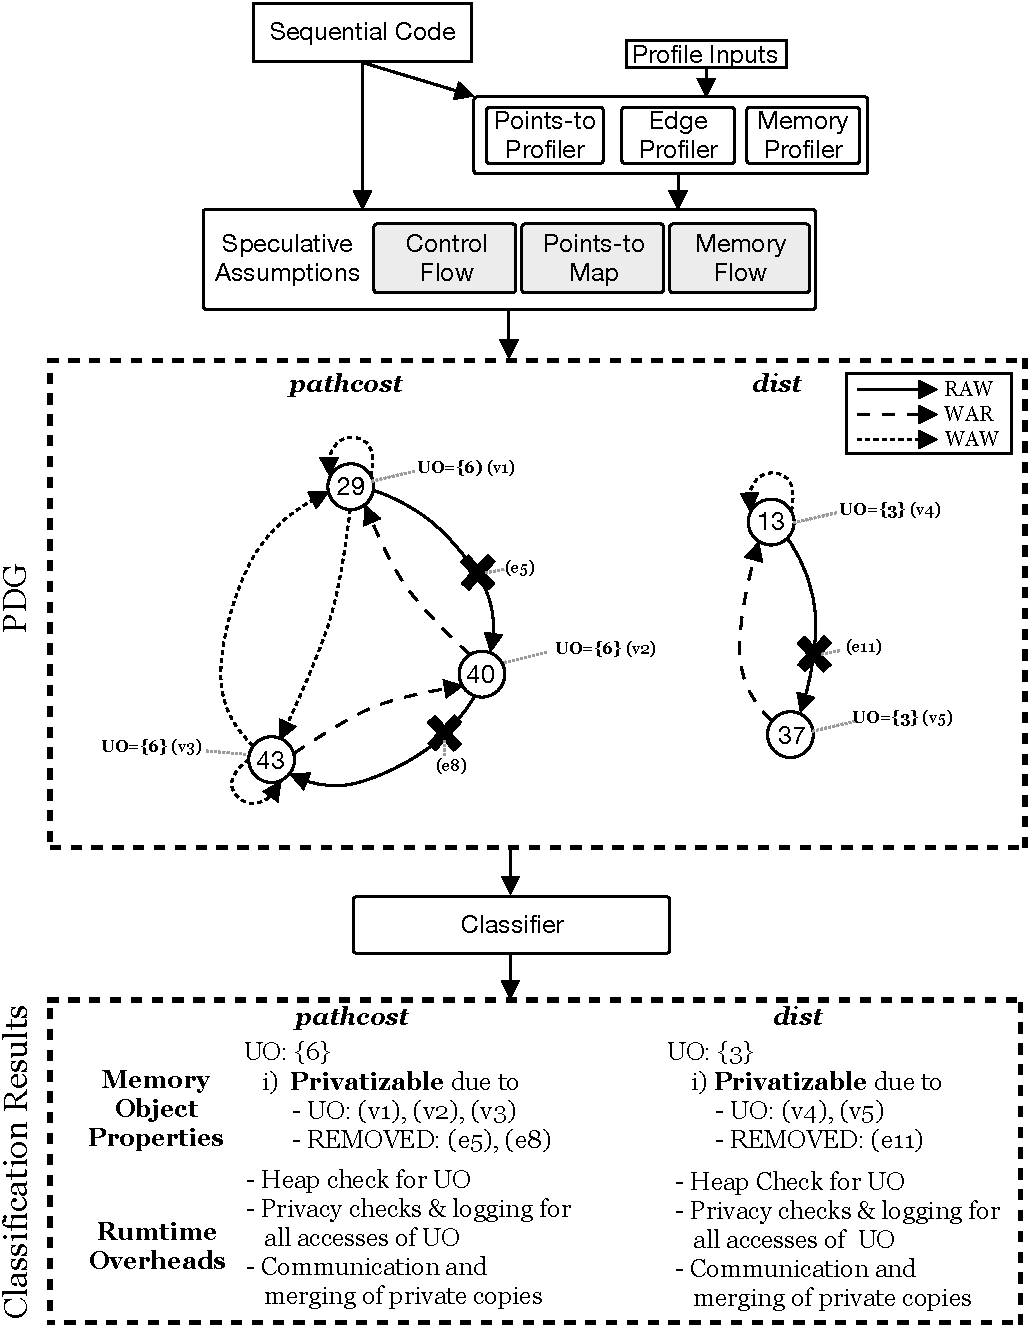
\includegraphics[width=0.46\textwidth]{figures/privateer-example-crop}
}
\qquad
\subfloat[This work]{
  \centering
  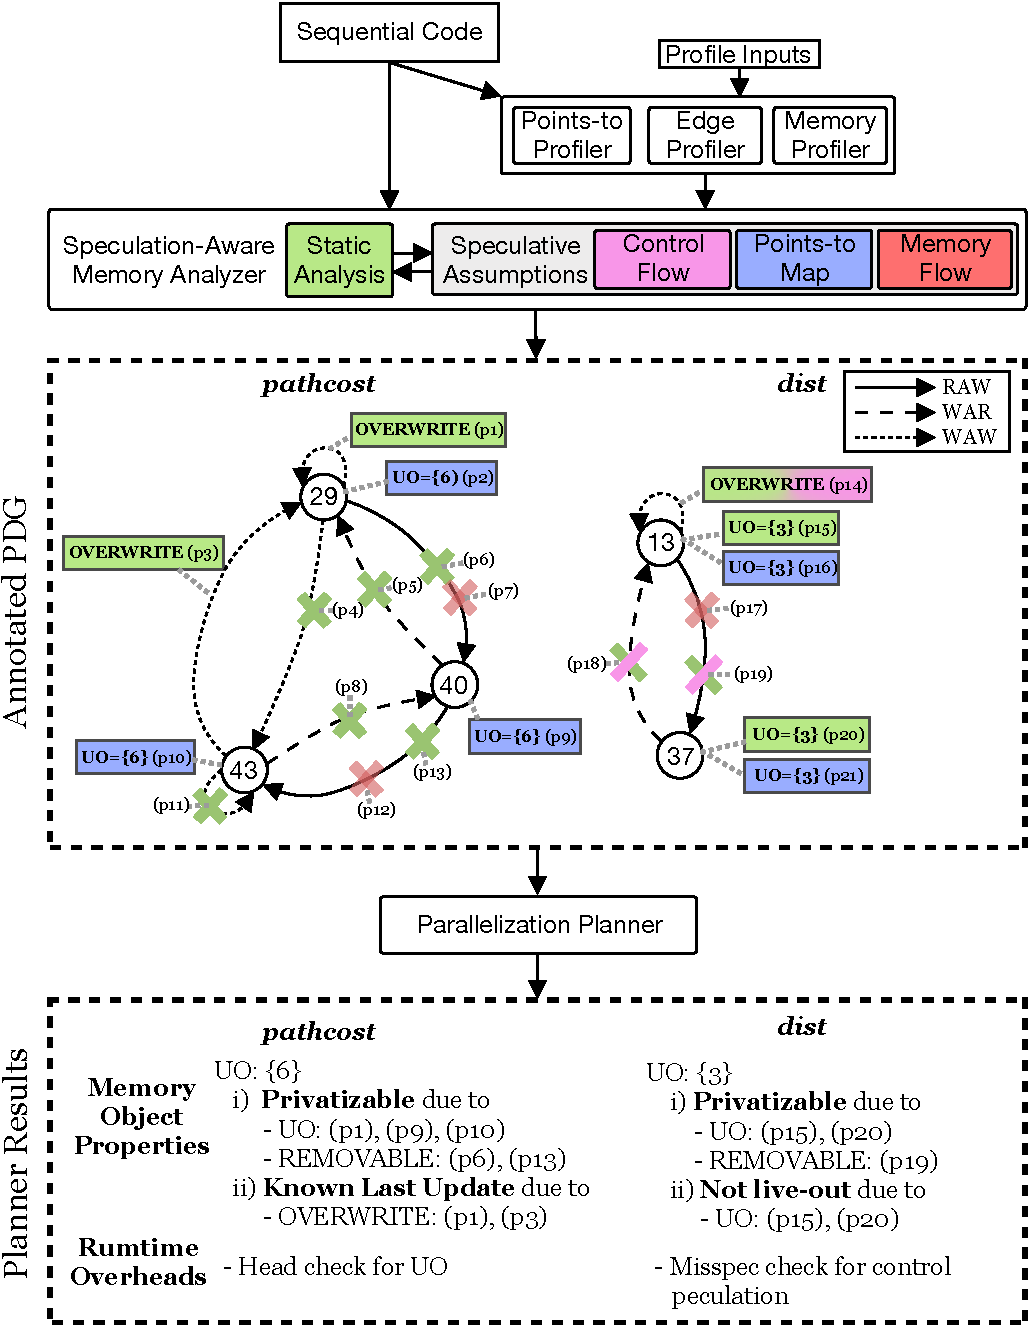
\includegraphics[width=0.46\textwidth]{figures/perspective-example-crop}
}
}
\caption{Comparison of Privateer with \name for handling memory
objects \textit{pathcost} and \textit{dist} of the hot loop of \textit{dijkstra}}
\label{fig:dijkstra_motivation_comparison}
\end{figure*}

\begin{figure*}[!b]
\centering
\scriptsize
\resizebox{0.8\linewidth}{!}{
\subfloat[Privateer~\cite{johnson:12:pdli}]{
  \centering
  \begin{minipage}{9.2cm}
  \begin{lstlisting}[morekeywords={pathcost}, belowskip=0pt, firstnumber=1,
name=dij_checks]
int *pathcost; // dyn alloc 1-D N
int *adj; // dyn alloc 2-D NxN
int dist, v, src, i;

for (src=0; src<N; src++) {
\end{lstlisting}

\begin{lstlisting}[morekeywords={pathcost}, aboveskip=0pt,belowskip=0pt,backgroundcolor=\color{lightgray},
firstnumber=auto, name=dij_checks]
  // Privacy Check
  private_write(pathcost, N*sizeof(int));
\end{lstlisting}

\begin{lstlisting}[morekeywords={pathcost},aboveskip=0pt, belowskip=0pt, firstnumber=auto,name=dij_checks]
  for (i=0; i<N; i++)
    pathcost[i] = inf;

  enqueue(src, 0);
  while (!emptyQ()) {
    dequeue(&v, &dist);
    for (i=0; i<N; i++) {
      nDist = adj[v][i] + dist;
\end{lstlisting}

\begin{lstlisting}[morekeywords={pathcost}, aboveskip=0pt,belowskip=0pt,backgroundcolor=\color{lightgray},
firstnumber=auto, name=dij_checks]
      // Privacy Check
      private_read(pathcost, sizeof(int));
\end{lstlisting}


\begin{lstlisting}[morekeywords={pathcost}, aboveskip=0pt, belowskip=0pt, firstnumber=auto,name=dij_checks]
      if (pathcost[i] > nDist) {
\end{lstlisting}

\begin{lstlisting}[morekeywords={pathcost}, aboveskip=0pt,belowskip=0pt,backgroundcolor=\color{lightgray},
firstnumber=auto, name=dij_checks]
        // Privacy Check
        private_write(pathcost, sizeof(int));
\end{lstlisting}

\begin{lstlisting}[morekeywords={pathcost}, aboveskip=0pt, belowskip=0pt, firstnumber=auto,name=dij_checks]
        pathcost[i] = nDist;
        enqueue(i, nDist);
      }
    }
  }
}
\end{lstlisting}

  \end{minipage}
}
\qquad
\qquad
\subfloat[This work]{
  \centering
  \begin{minipage}{7cm}
  %\begin{lstlisting}[morekeywords={pathcost}, belowskip=0pt, firstnumber=1,
%name=dij_checks]
%int *pathcost; // dyn alloc 1-D N
%int *adj; // dyn alloc 2-D NxN
%int dist, v, src, i;


\begin{lstlisting}[morekeywords={pathcost,dist}, belowskip=0pt,
firstnumber=10, name=dij_checks, showlines=true]
int dequeue() {
  if (!emptyQ()) {


\end{lstlisting}

\begin{lstlisting}[morekeywords={pathcost,dist}, aboveskip=0pt, belowskip=0pt,
firstnumber=13, name=dij_checks]
    dist = ...
    ...
  }
\end{lstlisting}

  \begin{lstlisting}[morekeywords={pathcost}, aboveskip=0pt,belowskip=0pt,backgroundcolor=\color{lightgray}, firstnumber=auto, name=dij_checks]
  else // 0% added overhead
    misspec("Control misspec in dequeue()");
\end{lstlisting}

\begin{lstlisting}[morekeywords={pathcost,dist}, aboveskip=0pt, belowskip=0pt,
firstnumber=auto, name=dij_checks,showlines=true]
}

void worker_loop(int start, int N, int step) {

\end{lstlisting}

  \begin{lstlisting}[morekeywords={pathcost}, aboveskip=0pt,belowskip=0pt,backgroundcolor=\color{lightgray},
  firstnumber=auto, name=dij_checks,showlines=true]
  // Separation Local Check -- < 0.001% added overhead
  check_heap(pathcost, OVERWRITE_PRIVATE);
  \end{lstlisting}

\begin{lstlisting}[morekeywords={pathcost}, aboveskip=0pt,
belowskip=0pt, firstnumber=24,name=dij_checks,showlines=true]

  for (src=start; src<N; src+=step) {


\end{lstlisting}
\begin{lstlisting}[morekeywords={pathcost,dist}, aboveskip=0pt,
belowskip=0pt, firstnumber=28,name=dij_checks,showlines=true]
    for (i=0; i<N; i++)
      pathcost[i] = inf;

    enqueue(src, 0);
    while (!emptyQ()) {
      int v = dequeue();
      for (i=0; i<N; i++) {
\end{lstlisting}
\begin{lstlisting}[morekeywords={pathcost,dist,nDist}, aboveskip=0pt,
belowskip=0pt, firstnumber=auto,name=dij_checks,showlines=true]



        nDist = adj[v][i] + dist;
\end{lstlisting}
\begin{lstlisting}[morekeywords={pathcost}, aboveskip=0pt,
belowskip=0pt, firstnumber=auto,name=dij_checks,showlines=true]


        if (pathcost[i] > nDist) {


\end{lstlisting}
\begin{lstlisting}[morekeywords={pathcost}, aboveskip=0pt,
belowskip=0pt, firstnumber=auto,name=dij_checks]
          pathcost[i] = nDist;
          enqueue(i, nDist);
        }
      }
    }
\end{lstlisting}

\begin{lstlisting}[morekeywords={pathcost,dist}, aboveskip=0pt,
belowskip=0pt, firstnumber=auto,name=dij_checks,showlines=true]
  }
\end{lstlisting}

\begin{lstlisting}[morekeywords={pathcost},
aboveskip=0pt,belowskip=0pt,backgroundcolor=\color{lightgray},
firstnumber=auto, name=dij_checks,showlines=true]
  // only last iter's pathcost array
  // needs to be communicated -- < 1% added overhead
  if (src == N-1+step)
    communicate_pathcost();
\end{lstlisting}

\begin{lstlisting}[morekeywords={pathcost}, aboveskip=0pt,
belowskip=0pt, firstnumber=auto,name=dij_checks]
}
\end{lstlisting}

  \end{minipage}
}
}
\caption{Source code comparison of Privateer with \name for parallelized hot loop
of \textit{dijkstra}. Logging and checks
during loop execution dominate the overheads.}
\label{fig:dijkstra_motivation_comparison_source_code}
\end{figure*}
%caption,
%Checkpointing occurs every several (long running) loop iterations, thus its
%overhead is negligeable for \textit{dijkstra}.


\subsection{Example}
\label{motiv_example}

This example underlines inefficiencies and limitations of prior work
and showcases how the contributions of this paper enable more scalable
speculative parallelization.
%
Consider again the code in Figure~\ref{fig:dijkstra_motivation},
briefly discussed~\ref{motiv_overheads}.
%
Privatization enables parallelization by addressing cross-iteration
false dependences introduced by the reuse of \textit{pathcost} array,
and global variables \textit{nDist} and \textit{dist}.
%
From prior work, Privateer~\cite{johnson:12:pldi} is the only
automatic system to support privatization of dynamically allocated
objects, like \textit{pathcost}, even in the presence of unrestricted
pointers.

Figure~\ref{fig:dijkstra_motivation_comparison} compares the
compilation flow of \name with Privateer for handling memory objects
%for privatizing
\textit{pathcost} and \textit{dist}.
%
Privateer relies on profile information to infer that these two
objects are privatizable and is forced to apply transformations with
high runtime overheads.
%Even if memory analysis was used instead of memory speculation, the
%classifier sees the optimistic view of the program
%
On the other hand, \name employs an exploration phase that yields a
much more profitable plan.
%The PDG is annotated by the speculation-aware memory
Notice how the PDG is annotated with properties and underlying
speculative assumptions by the speculation-aware memory analyzer.
%
Just removing dependences in the PDG creates ambiguity on how a
dependence can be resolved, leading to over-speculation. The PDG
contains useful properties even for non-removable dependences. For
example, non-removable WAW edges in this example are annotated with
the \textit{overwrite} property that indicates that the destination
operation always overwrites the footprint of the source operation.
%
Based on the information on the PDG, three different transformations
offer handling of memory objects. Their offers specify the set of
speculative assumptions that are required for the transformation to be
applicable.
%For example, handling of \textit{dist} requires usage of control
%speculation (for the branch in line 11,
%fig.~\ref{fig:dijkstra_motivation}).
%
%Notice that \textit{dist} can be handled by all three
%transformations.
%
The DOALL planner then selects the lowest cost solution for each
memory object. For example, for \textit{dist} the local
privatization's offer is selected since it is the cheapest
privatization transformation and it requires a speculative assumption
that other options require as well. \textit{nDist} object (not shown
in this figure) is also handled by local privatization.
%
Extracting this efficient plan would not be possible without the use
speculation-aware memory analyzer and efficient speculative
privatization transformations.

%Notice that speculation-aware memory analyzer allows removal of the
%RAW dependence between instruction 13 and 37 with a combination of
%static analysis and control speculation. This dependence would require
%usage of memory speculation in prior.
%not only in Privateer but in any other automatic parallelization
%speculative system.


%Whilst the private property is enough for DOALL
%Notice that we infer an additional property that improves the profitability
%of parallelization.

%For inferring the property that a private memory object has the additional local-private
%property, it suffices to identify all accesses of the memory object
%and check that all of them are within the loop.
%locally-accessed property.


Figure~\ref{fig:dijkstra_motivation_comparison_source_code} compares
the resulting parallelized versions (in a simplified form) for
Privateer and \namensp. The code includes all the added checks,
logging and handling live-out overheads. The code changes are marked
with the average added overhead over the useful work of each worker.
It is clear that Privateer introduces a lot of added overhead
considerably limiting its profitability. \namensp, on the other hand,
thanks to the use of speculative-aware memory analyzer, careful
selection of applied transformations, and use of efficient
privatization variants is able to parallelize dijkstra with minimum
overheads. In fact, \name exhibits 4.8$\times$ speedup over Privateer
for dijkstra (see~\ref{eval}).


%Privateer would choose to just do simple privatization with mem spec.
%The spec-aware analyzer allows removal of mem spec and efficient
%privatization in this case.
%
%\begin{itemize}
%\item
%Privatization of these memory objects requires:
%\begin{enumerate}
%\item
%identification of all accesses of these objects
%    within the loop
%\item
%absence of cross-iteration flow
%     dependences on each of these accesses
%\end{enumerate}
%
%\end{itemize}
%
%
%DOALL can become applicable if these two objects are proven to have the
%private property.
%
%We compare our approach where we combine static analysis with cheap-to-validate
%with privateer's monolithic approach that over-speculates and is limited by high
%runtime overheads.
%
%Note that anti-dependences are ignored since both systems use
%process-based runtime systems.
